\section{Algorithm}
\begin{frame}{Implementation: Web Scrapping}
    % 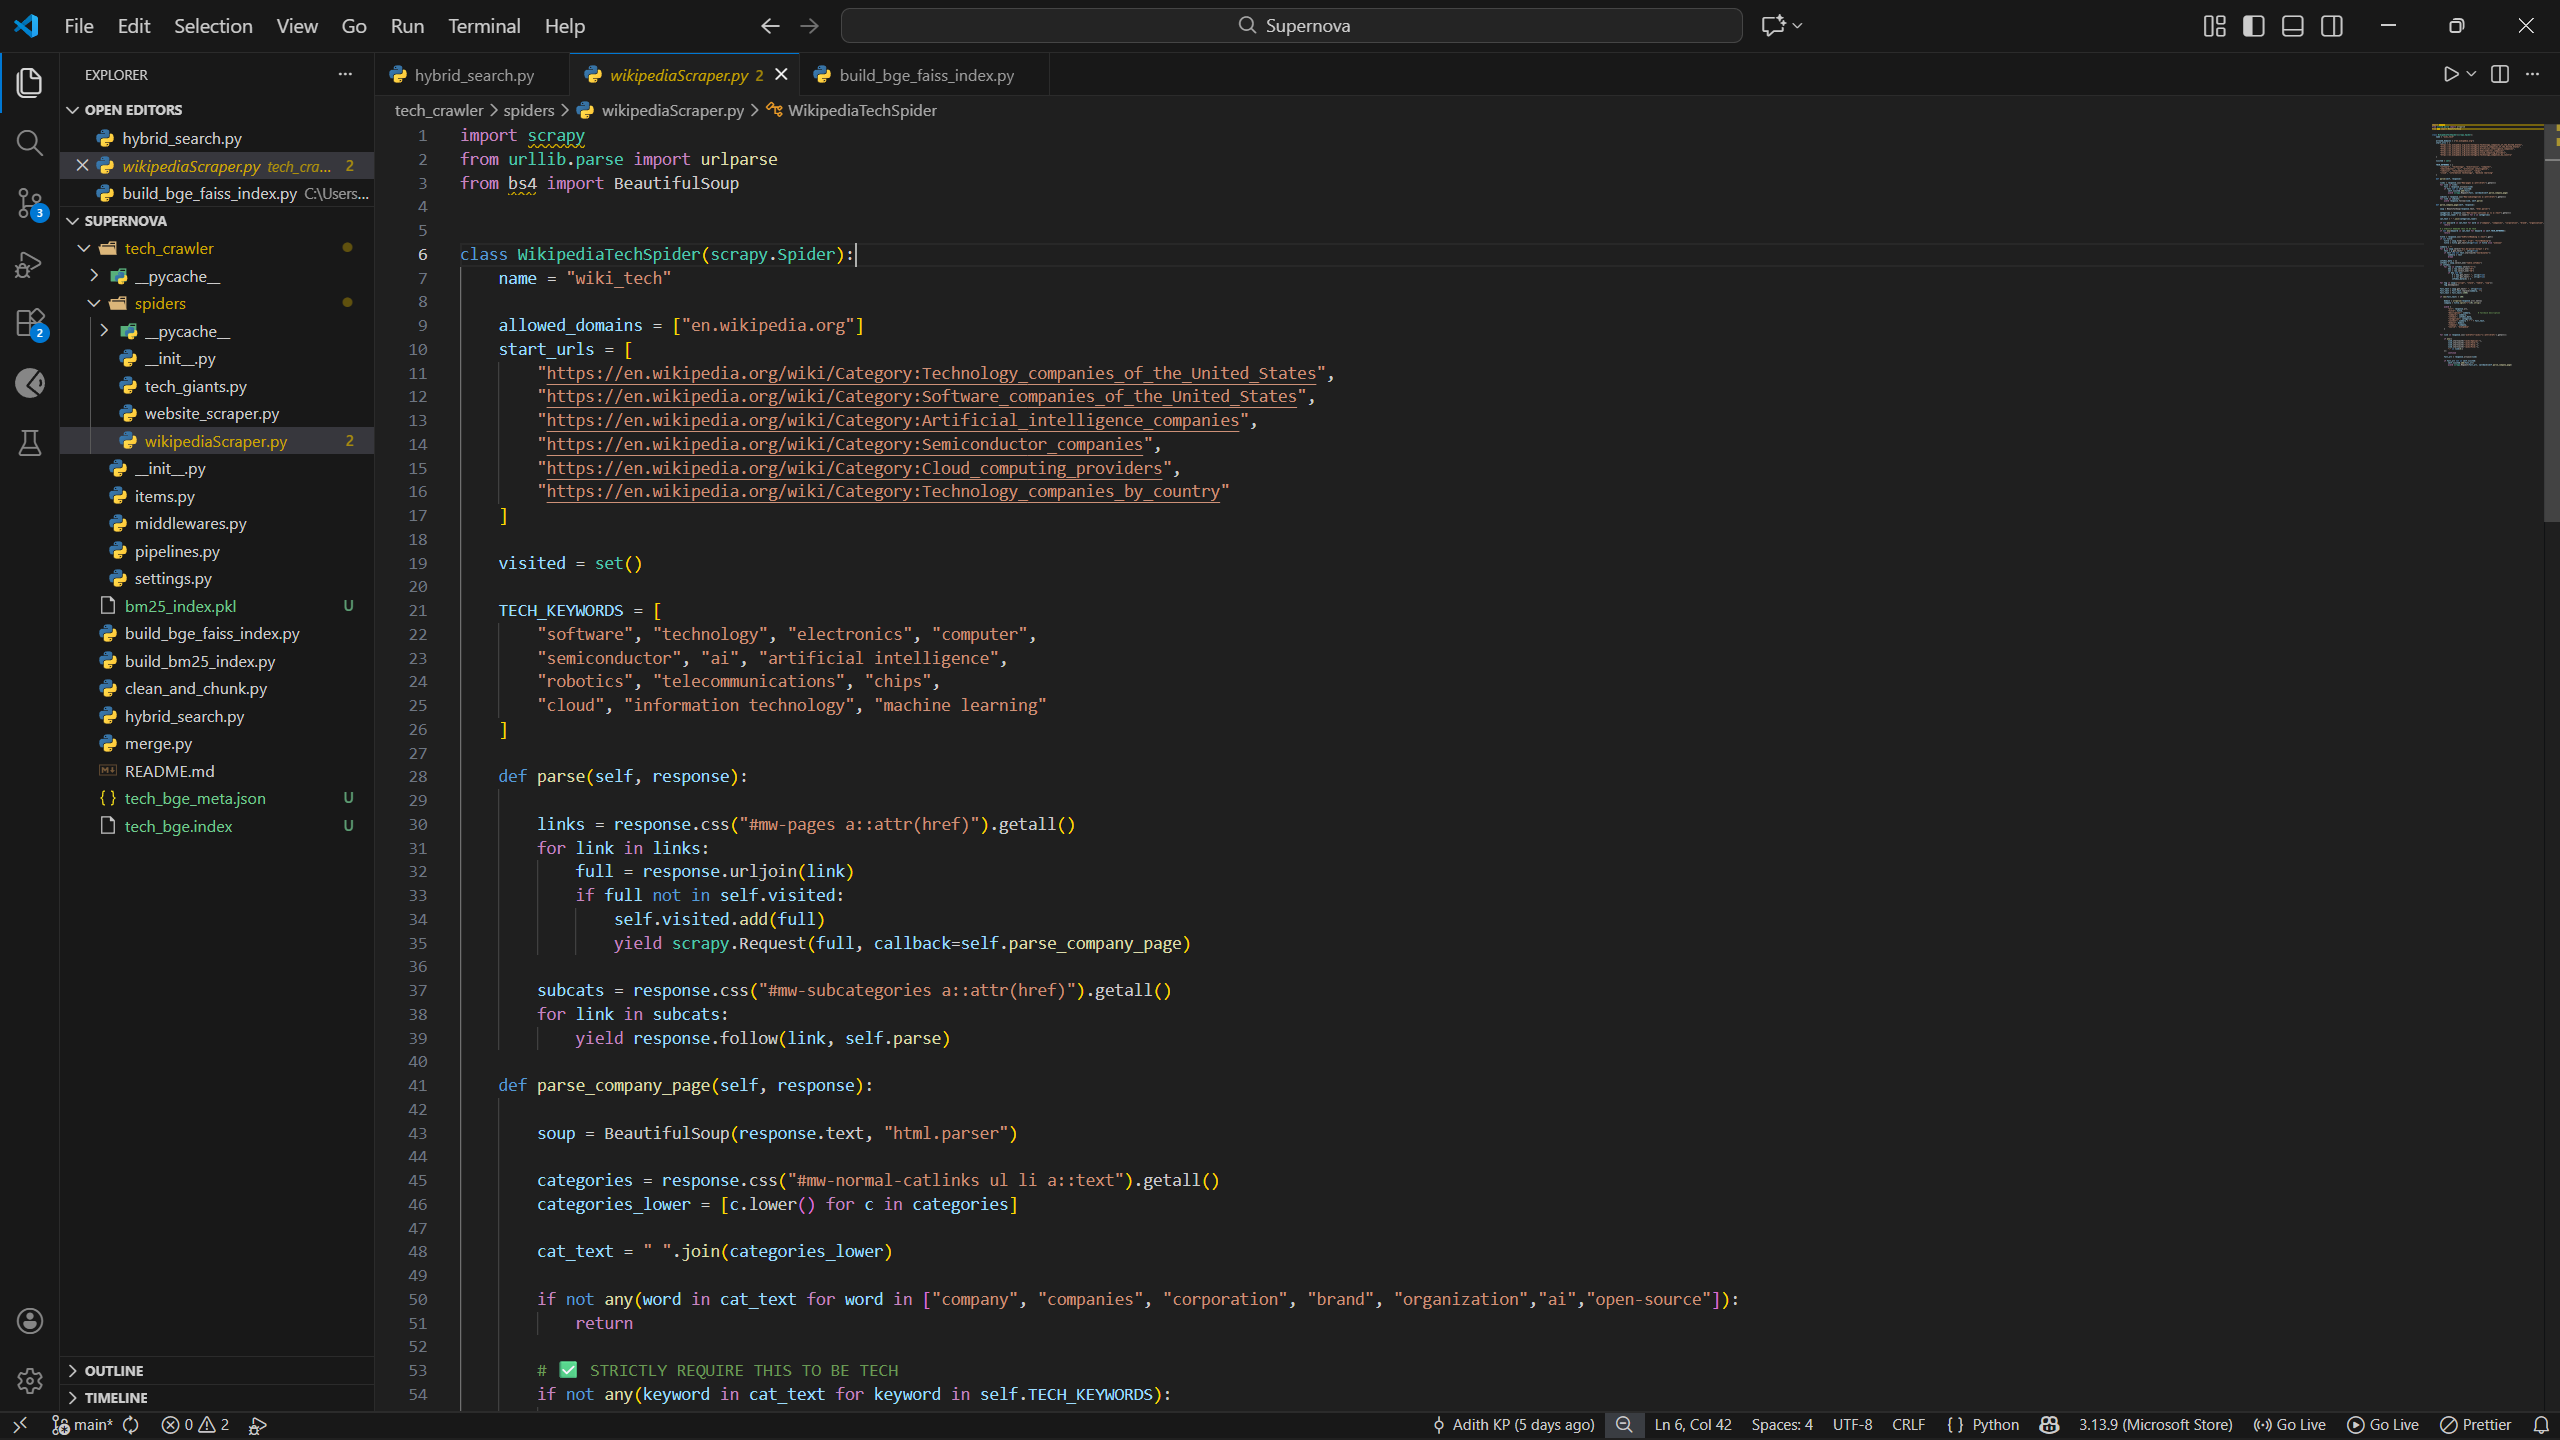
\includegraphics[width=1\textwidth,height=0.75\textheight,keepaspectratio]{slides/code1.png}
  
        \textbf{Step 1: Initialization:}
            \begin{itemize}
                \item[1.1] Specify the allowed domains along with the initial set of URLs to begin crawling.
                \item[1.2] Create and maintain a visited set in order to prevent repeated crawling of the same pages.
                \item[1.3] Define crawling limitations such as maximum depth and request delay.
            \end{itemize}
            
        
        \textbf{Step 2: Page Processing:}
            \begin{itemize}
            
                \item[2.1] Fetch a page from the start URLs.
                \item[2.2] Check if the page is valid and relevant.
                \item[2.3] Extract useful text and metadata.
                \item[2.4] Clean and structure the extracted content.
                \item[2.5] Store the processed data into the dataset.
            \end{itemize}
        
        \textbf{Step 3: Link Expansion:}
            \begin{itemize}
                \item[3.1] Identify and extract hyperlinks available on the page.
                \item[3.2] Filter the extracted links to retain only valid ones.
                \item[3.3] Continue processing newly obtained pages until the crawl limit is met.
            \end{itemize}
    
   
\end{frame}

\begin{frame}{Implementation: Data Merge:}
    % 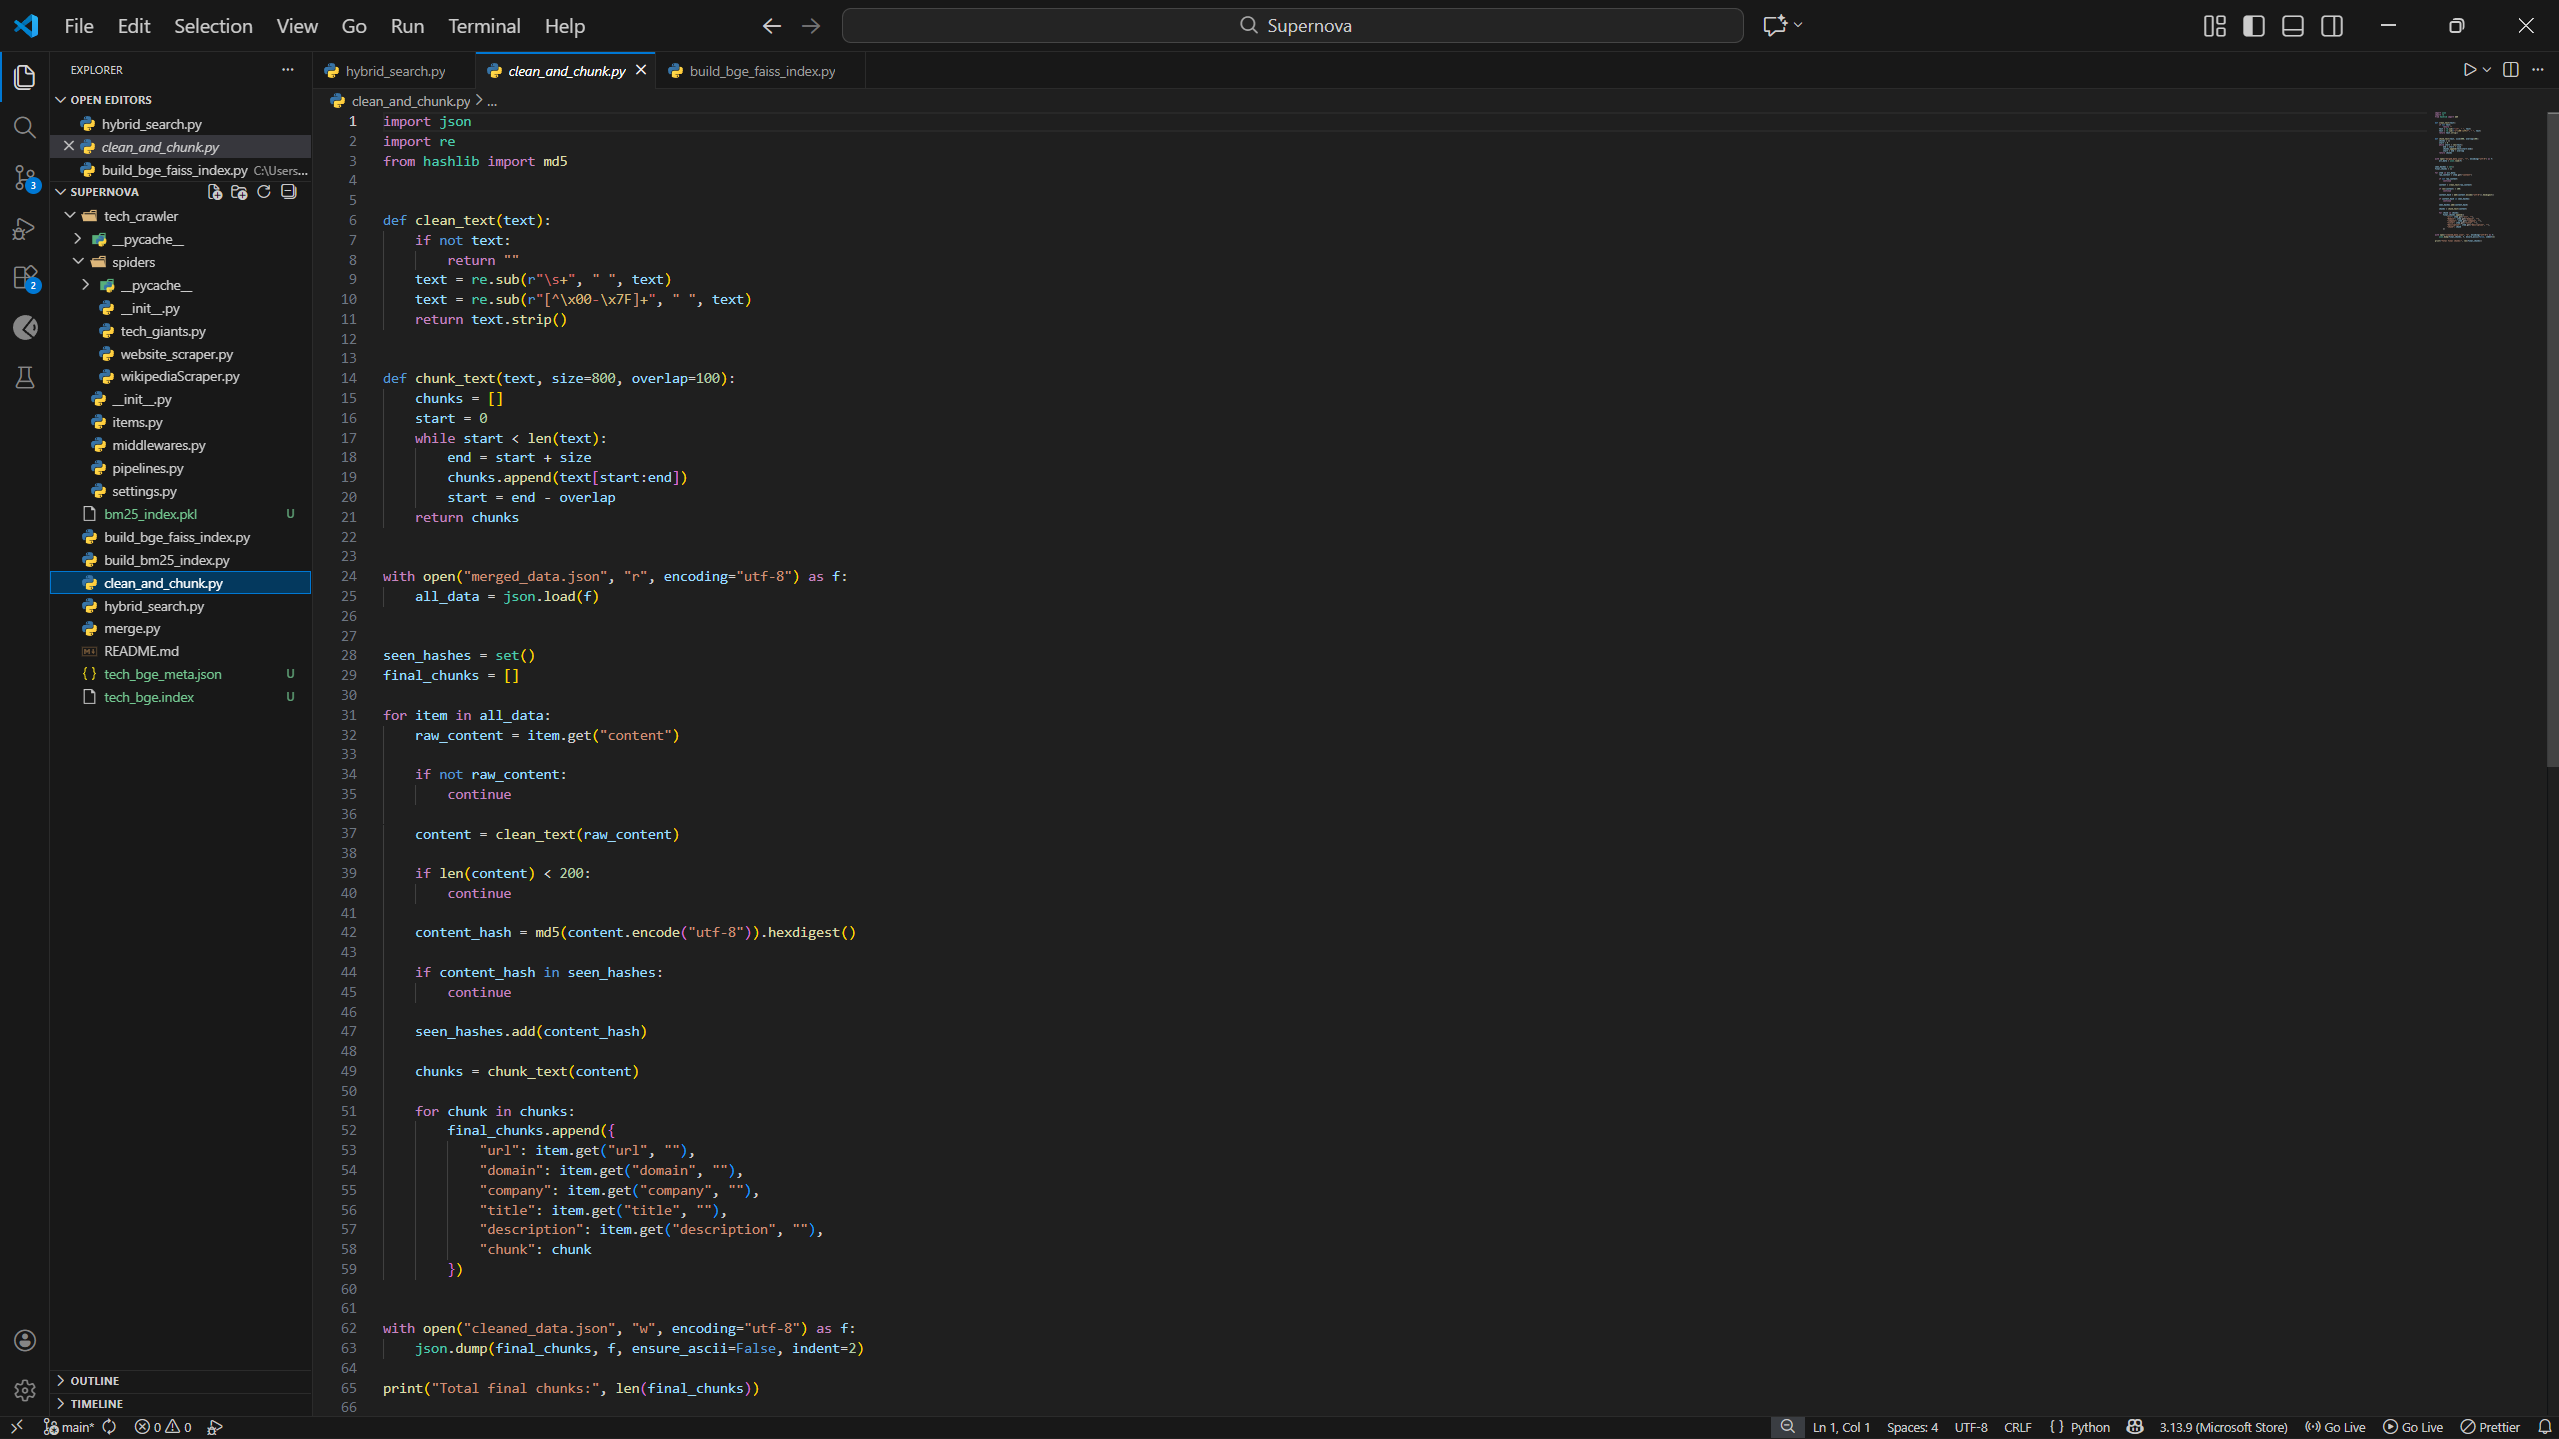
\includegraphics[width=1\textwidth,height=0.75\textheight,keepaspectratio]{slides/code2.png}
    \textbf{Step 4: Data Merge:}
        \begin{itemize}
        
            \item[4.1] Load datasets collected from different sources.
            \item[4.2] Combine all datasets into a single collection.
        
            \item[4.3] Normalize the data structure.
            \item[4.4] Ensure common fields such as:
                       (URL, Title, Content, Summary, Domain, Source)
        
            \item[4.5] Identify duplicate records based on URL or identifier.
            \item[4.6] Remove duplicate entries and retain unique records.
        
            \item[4.7] Finalize and prepare the unified dataset for further processing.
            \item[4.8] Store the merged dataset.
        
        \end{itemize}
        
        \textbf{Output:} A single unified and duplicate-free knowledge base.

\end{frame}

\begin{frame}{Implementation: Cleaning \& Chunking: }
    % 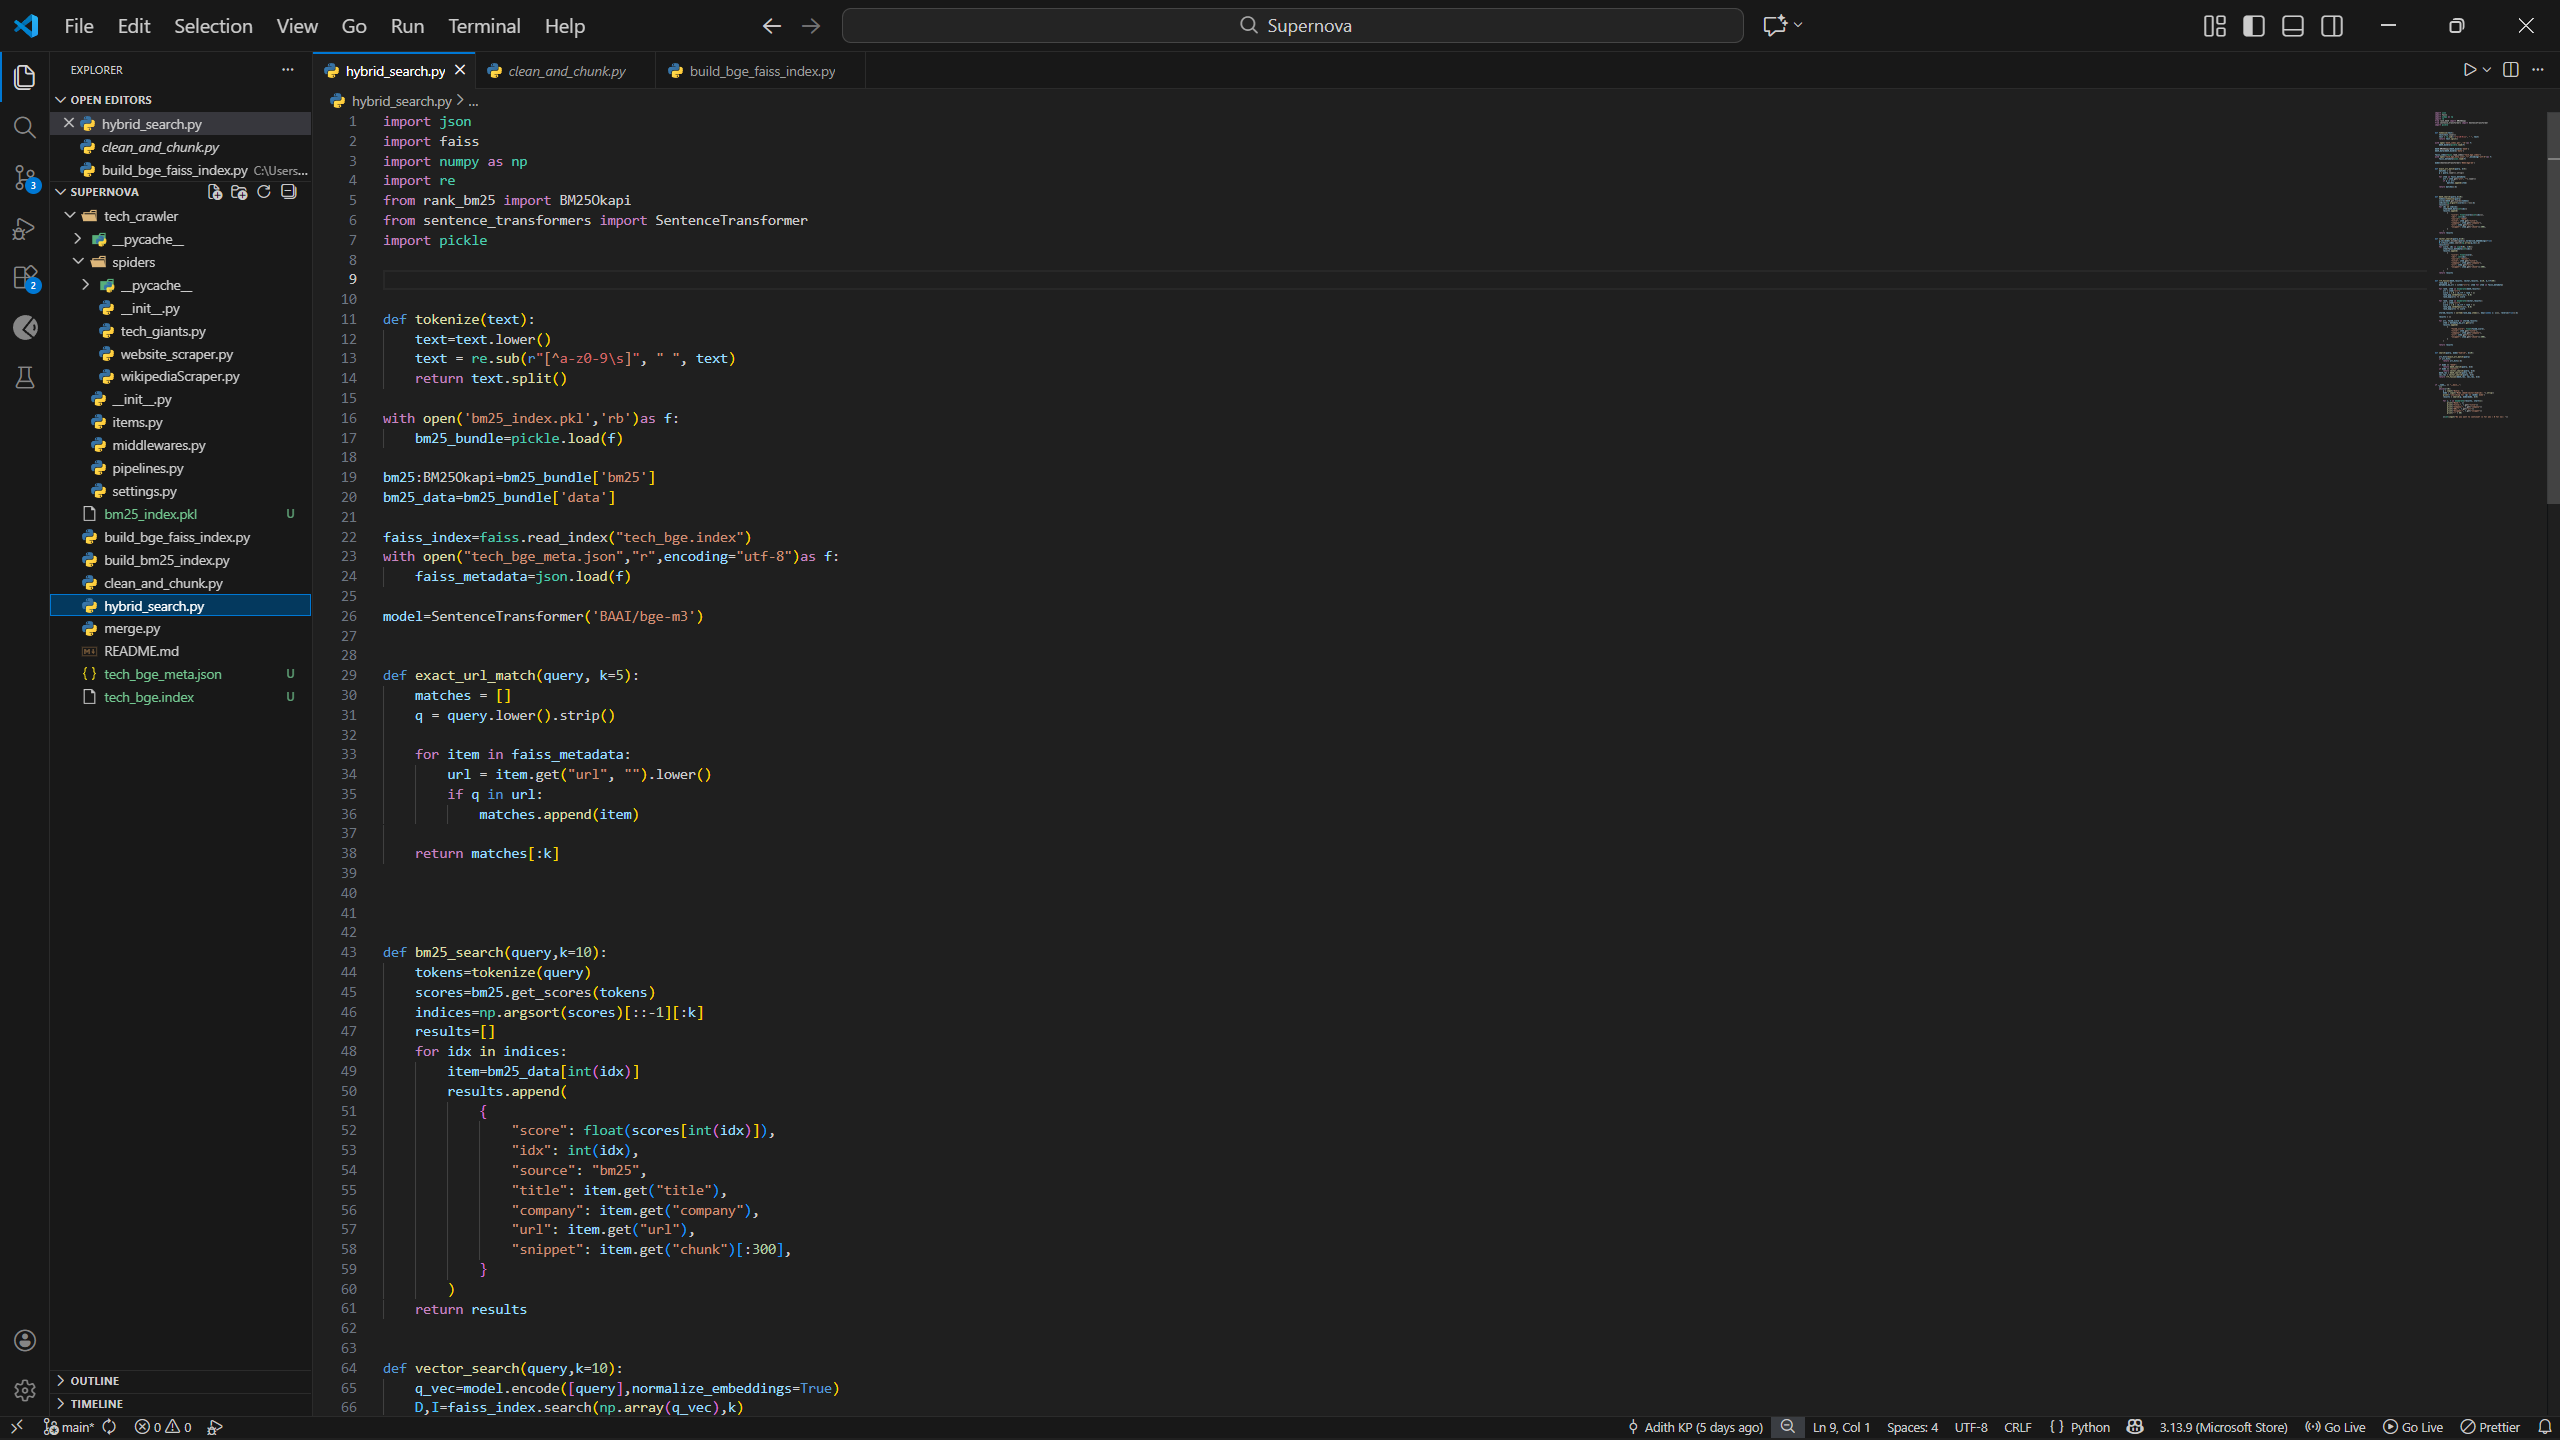
\includegraphics[width=1\textwidth,height=0.75\textheight,keepaspectratio]{slides/code3.png}
    \textbf{Step 5: Cleaning and Chunking:}
    \begin{itemize}
    
        \item[5.1] Load the merged dataset containing all documents.
    
        \item[5.2] Perform text cleaning for each document:
              \begin{itemize}
                  \item[5.2.1] Remove unwanted symbols and noisy characters.
                  \item[5.2.2] Normalize whitespace and formatting.
                  \item[5.2.3] Retain only meaningful readable content.
              \end{itemize}
    
        \item[5.3] Validate content quality:
              \begin{itemize}
                  \item[5.3.1] Discard documents with insufficient content length.
                  \item[5.3.2] Remove duplicate or redundant content.
              \end{itemize}
    
        \item[5.4] Perform text chunking:
              \begin{itemize}
                  \item[5.4.1] Split large documents into smaller chunks.
                  \item[5.4.2] Maintain slight overlap between consecutive chunks to preserve context.
              \end{itemize}
    
        \item[5.5] Attach necessary metadata for each chunk
                  (URL, title, domain, source information, etc.).
    
        \item[5.6] Store the cleaned and chunked dataset for further processing.
    
    \end{itemize}
    
    \textbf{Output:} Clean, context-preserved, and chunked dataset ready for indexing.

\end{frame}

\begin{frame}{Implementation: BM25 Indexing:}
    % 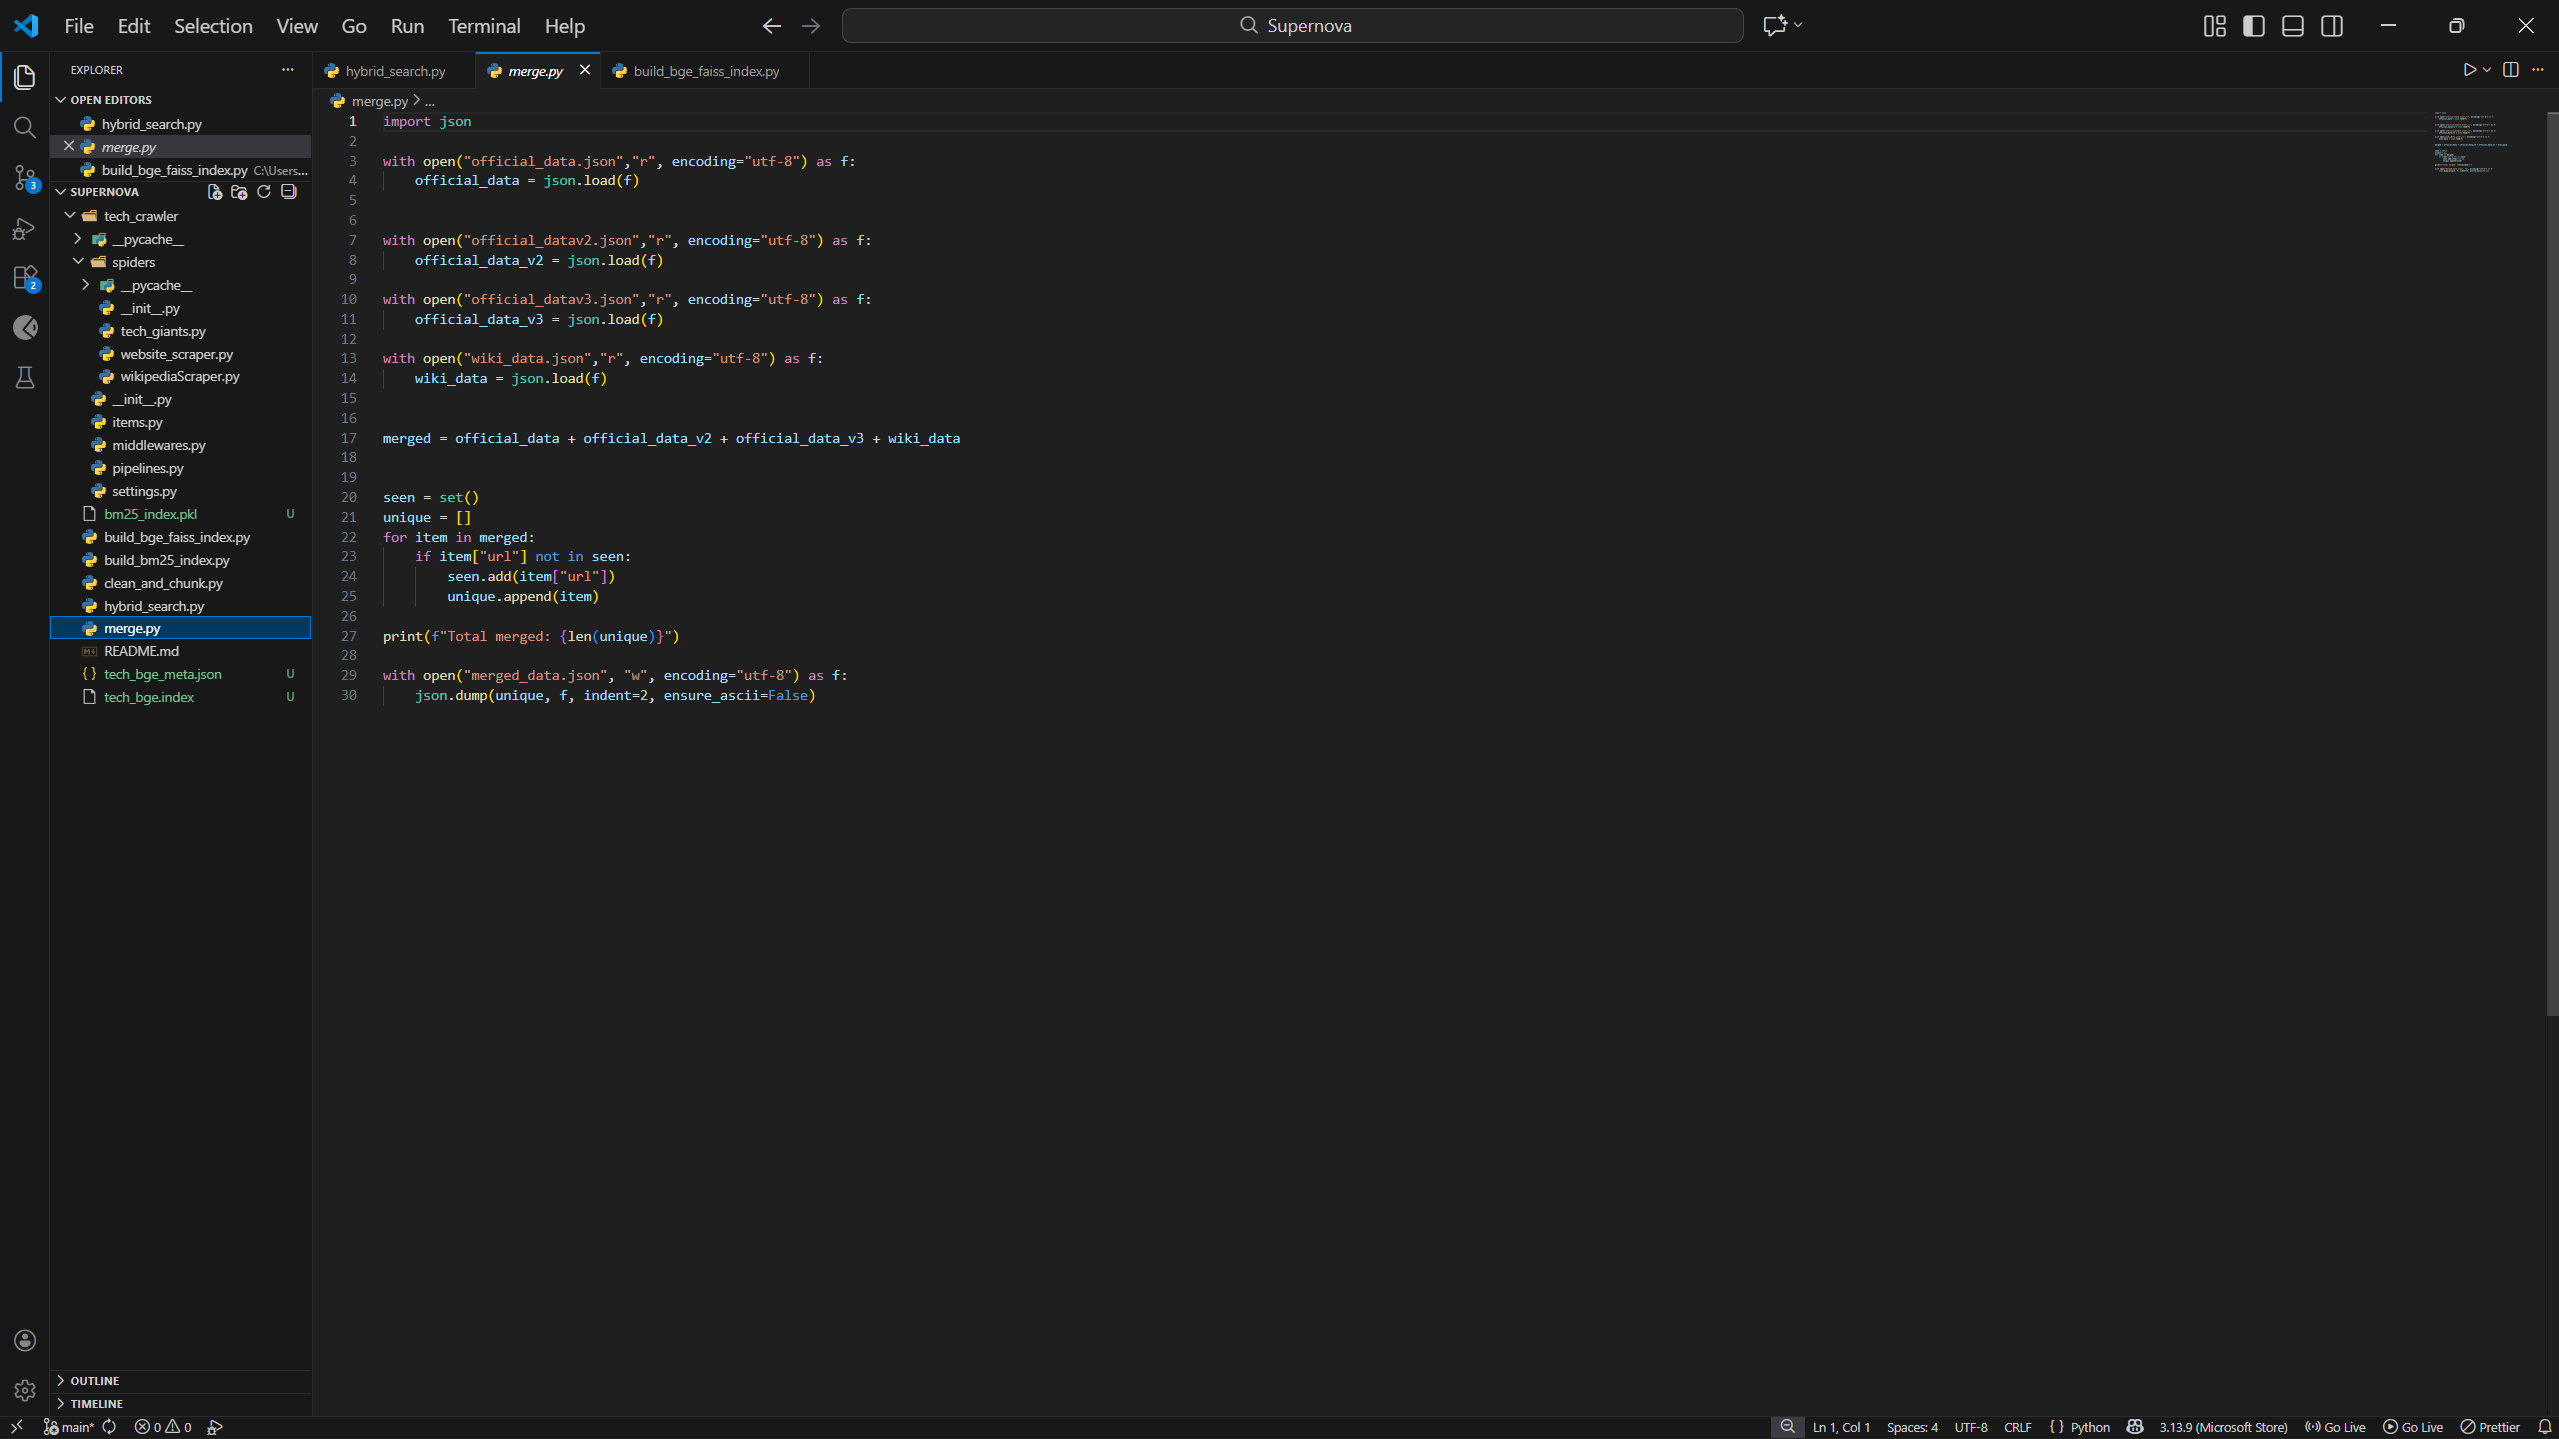
\includegraphics[width=1\textwidth,height=0.75\textheight,keepaspectratio]{slides/code4.png}
    \textbf{Step 6: BM25 Indexing:}
    \begin{itemize}
    
        \item[6.1] Load the cleaned and chunked dataset.
    
        \item[6.2] Prepare the text corpus:
              \begin{itemize}
                  \item[6.2.1] Convert text to lowercase.
                  \item[6.2.2] Remove unwanted characters and symbols.
                  \item[6.2.3] Tokenize text into individual terms.
              \end{itemize}
    
        \item[6.3] Construct the BM25 index using the tokenized corpus.
    
        \item[6.4] Store the BM25 model along with corresponding document chunks.
    
        \item[6.5] Confirm successful index creation
                  and record the total number of indexed documents.
    
    \end{itemize}
    
    \textbf{Output:} BM25 lexical index ready for efficient keyword-based retrieval.

\end{frame}

\begin{frame}{Implementation: BGE M3 Embedding Index:}
    % 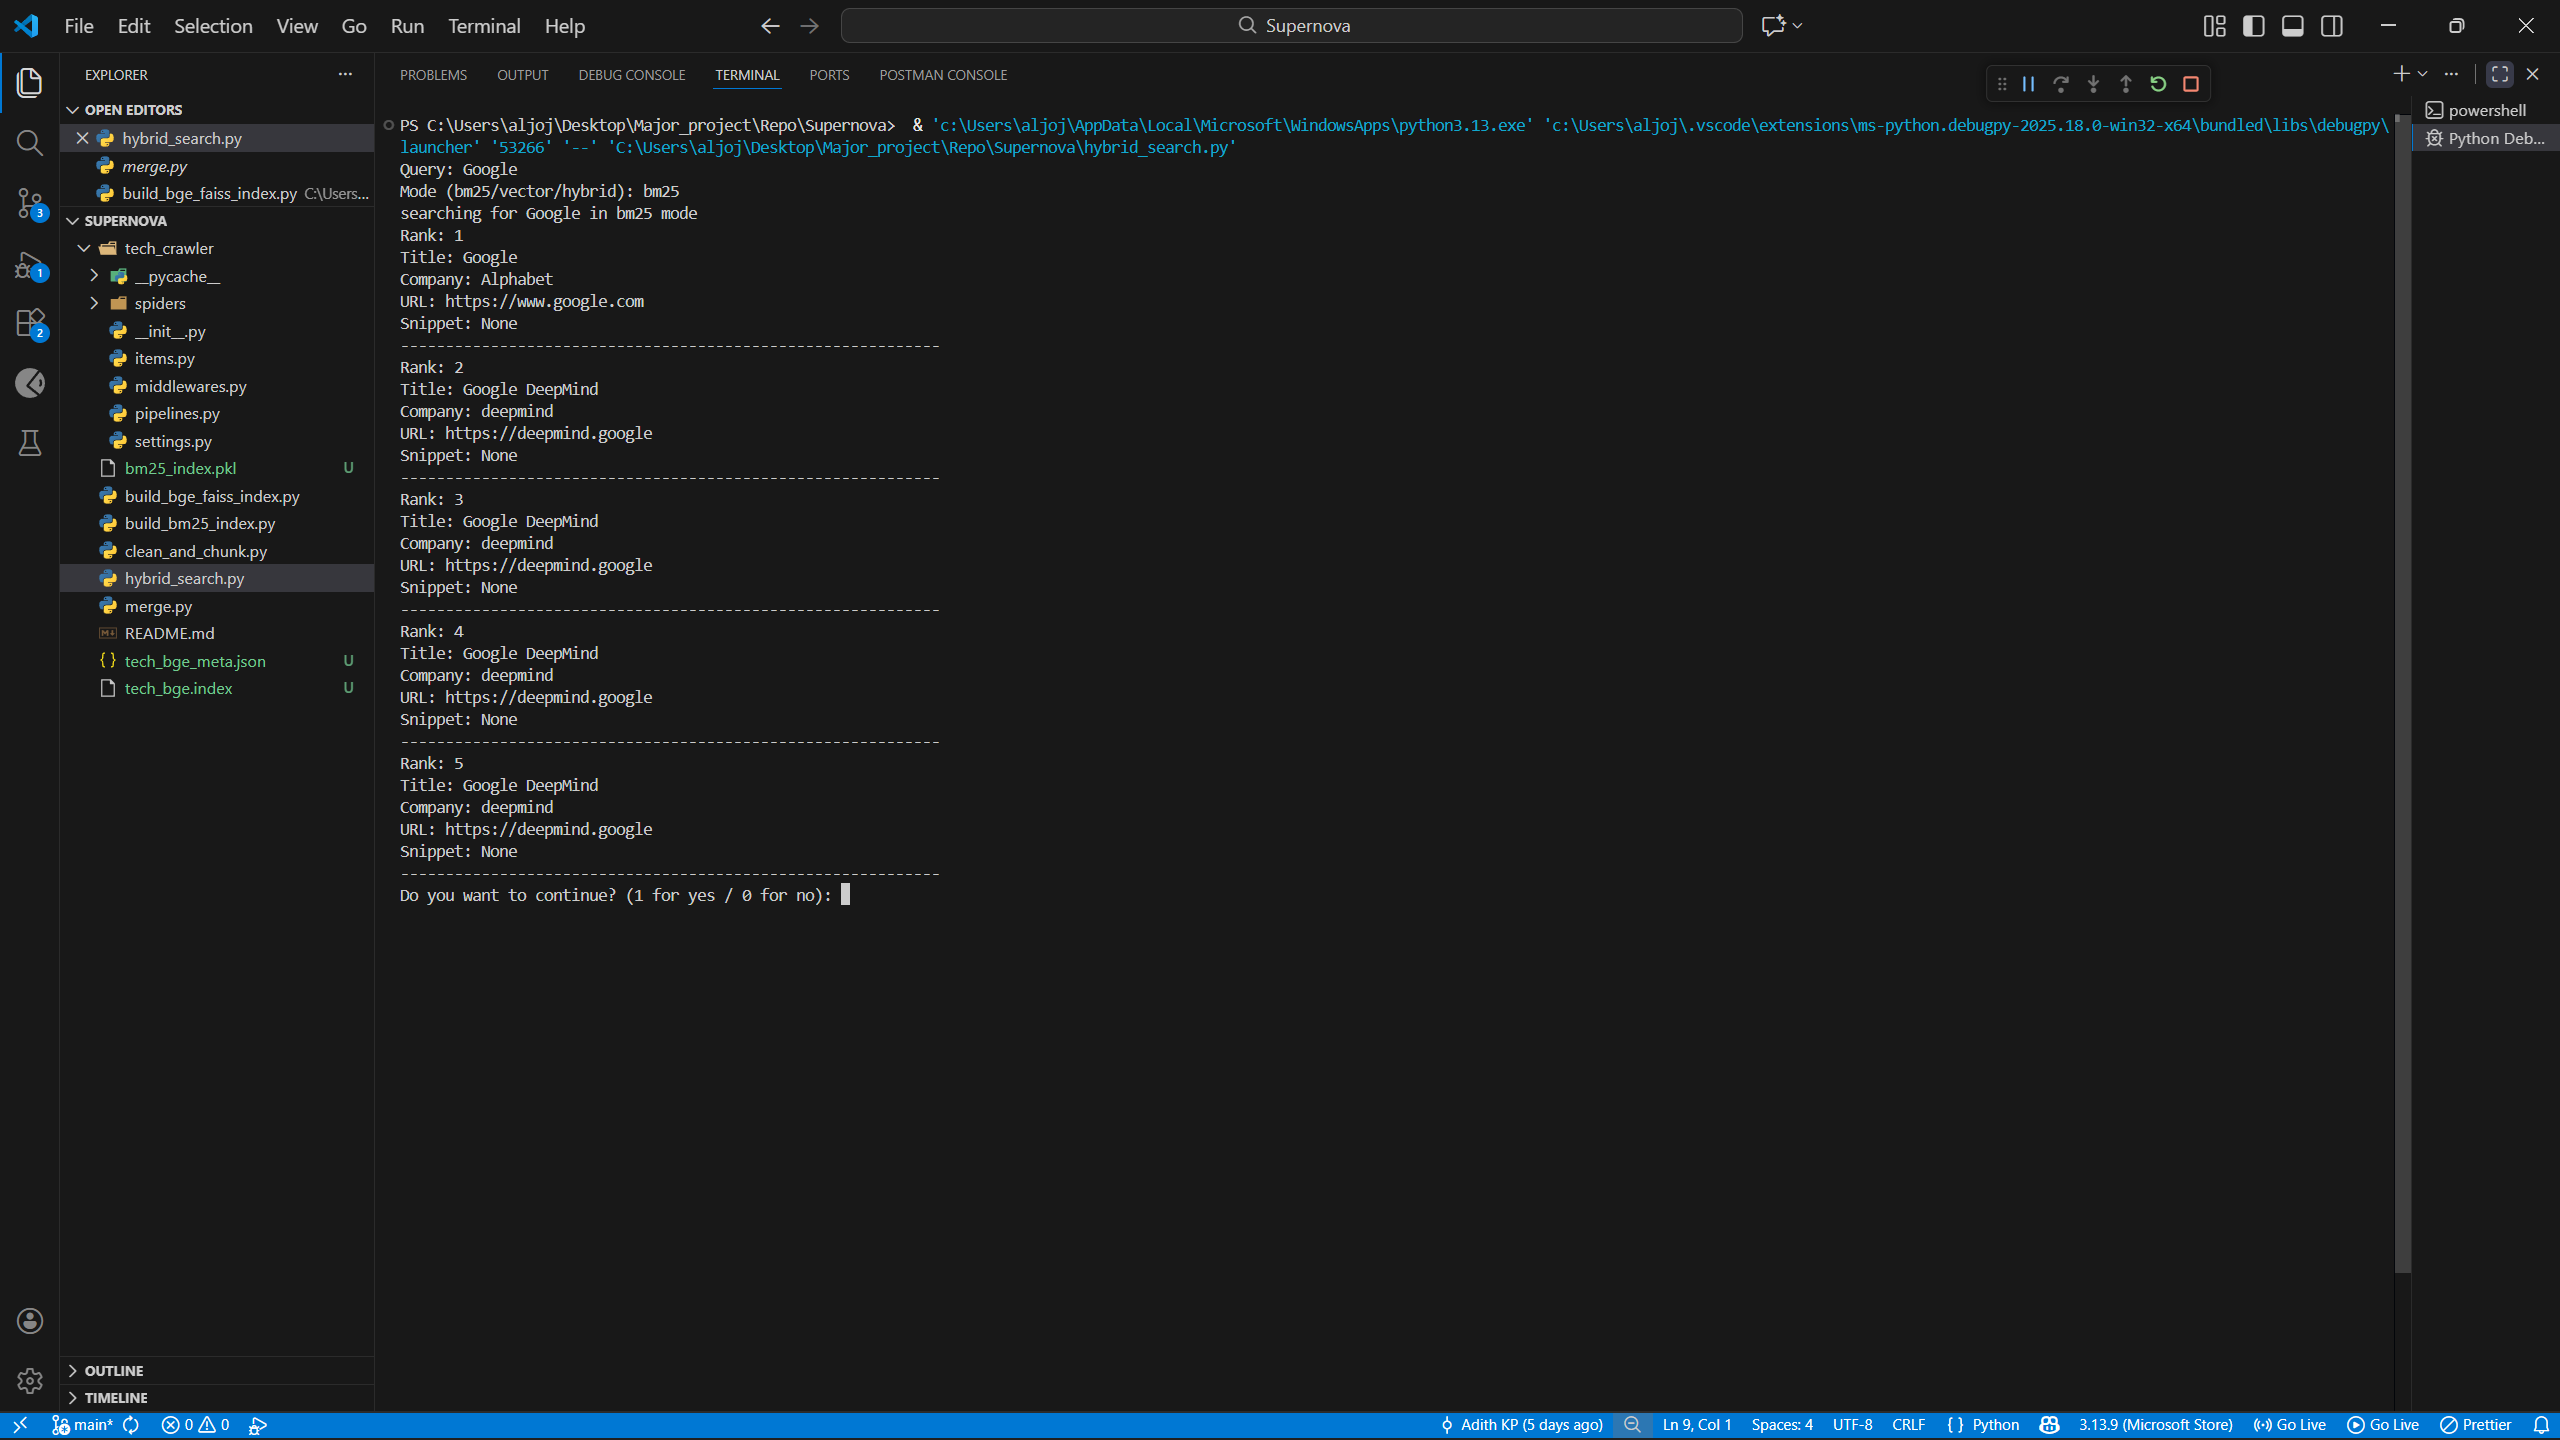
\includegraphics[width=1\textwidth,height=0.75\textheight,keepaspectratio]{slides/output1.png}
    \textbf{Step 7: BGE-M3 Semantic Embedding Index:}
    \begin{itemize}
    
        \item[7.1] Load the cleaned and chunked dataset.
    
        \item[7.2] Initialize the BGE-M3 sentence embedding model.
    
        \item[7.3] Prepare text for embedding:
              \begin{itemize}
                  \item[7.3.1] Extract text chunks from the dataset.
                  \item[7.3.2] Convert each chunk into a fixed-length vector
                                representation using the embedding model.
                  \item[7.3.3] Normalize embeddings to maintain consistency.
              \end{itemize}
    
        \item[7.4] Create a vector index:
              \begin{itemize}
                  \item[7.4.1] Determine embedding dimension.
                  \item[7.4.2] Initialize a similarity-based vector index.
                  \item[7.4.3] Insert all embeddings into the index.
              \end{itemize}
    
        \item[7.5] Store the semantic index along with metadata
                  for efficient retrieval during search operations.
    
        \item[7.6] Confirm successful creation of the index and
                  record total vectors stored.
    
    \end{itemize}

\textbf{Output:} A FAISS-based semantic vector index enabling efficient meaning-based retrieval.

\end{frame}

\begin{frame}{Implementation: Search Pipelines:}
    \textbf{Step 8: Search Pipeline:}
    \begin{itemize}
    
        \item[8.1] Load required components:
              \begin{itemize}
                  \item[8.1.1] Load BM25 lexical index.
                  \item[8.1.2] Load semantic embedding index.
                  \item[8.1.3] Load corresponding metadata.
              \end{itemize}
    
        \item[8.2] Accept user query input.

        \item[8.3] Identifies what the user want.

        \item[8.4] Orchestrator agent decides which agents to use. 
    
        \item[8.5] Perform preliminary matching:
              \begin{itemize}
                  \item[8.5.1] Check for direct or exact URL-related matches.
                  \item[8.5.2] If exact match found, return results immediately.
              \end{itemize}

        \item[8.6] Reformulate the query
    
        \item[8.7] Lexical Search (BM25):
              \begin{itemize}
                  \item[8.7.1] Tokenize and preprocess the query.
                  \item[8.7.2] Retrieve top-$k$ documents using BM25 scoring.
              \end{itemize}
    
        \item[8.8] Semantic Search (Vector Index):
              \begin{itemize}
                  \item[8.8.1] Convert query into embedding vector.
                  \item[8.8.2] Retrieve top-$k$ semantically similar documents.
              \end{itemize}
    \end{itemize}
\end{frame}

\begin{frame}{Implementation: Search Pipelines..}
    
    \begin{itemize}
       
        \item[8.9] Hybrid Retrieval using \textbf{RRF} Fusion:
              \begin{itemize}
                  \item[8.9.1] Combine BM25 and semantic results.
                  \item[8.9.2] Apply Reciprocal Rank Fusion to compute final ranking.
                  \item[8.9.3] Select top-$k$ ranked documents.
              \end{itemize}
    
        \item[8.10] Return the ranked results with title, source, URL, and snippet.
    
    \end{itemize}

\textbf{Output:} Final ranked search results using lexical, semantic, or hybrid retrieval.

    
\end{frame}

\begin{frame}{Implementation: Answer Generation:}
    \textbf{Step 9: Answer Generation:}
    \begin{itemize}
        \item[9.1] Load input parameters:
        \begin{itemize}
                  \item[9.1.1] Accept the original user query string.
                  \item[9.1.2] Accept the list of retrieved context documents.
                  \item[9.1.3] Accept optional original intent label (default: "Unknown").
                  \item[9.1.4] Accept optional reformulated query string (default: "None").
        \end{itemize}

        \item[9.2] Format retrieved context into structured string:
        \begin{itemize}
                  \item[9.2.1] Iterate over each retrieved document in the context list.
                  \item[9.2.2] Extract title, URL, and snippet fields from each document.
                  \item[9.2.3] Append each as a labelled source block (Source 1, Source 2, ...).
        \end{itemize}

        \item[9.3] Construct synthesis prompt:
        \begin{itemize}
                  \item[9.3.1] Inject original query, detected intent, and reformulated query into user context section.
                  \item[9.3.2] Inject formatted context string into search results section.
                  \item[9.3.3] Attach grounding instructions: answer only from context, cite sources, use Markdown, avoid hallucinations.
        \end{itemize}
        
    \end{itemize}
\end{frame}

\begin{frame}{Implementation: Answer Generation...}
    \begin{itemize}
        \item[9.4] Call \textbf{LLM} \textbf{API}
        \begin{itemize}
                  \item[9.4.1] Send constructed prompt as a user-role message.
                  \item[9.4.2] Receive completion response from the \textbf{API}.
        \end{itemize}

        \item[9.5] Extract and return generated answer:
        \begin{itemize}
                  \item[9.5.1] Parse first choice message content from \textbf{API} response.
                  \item[9.5.2] Strip leading/trailing whitespace.
                  \item[9.5.3] If context is insufficient, return: "I need more information to answer this query."
                  \item[9.5.4] Return final answer string in Markdown format.
                  
        \end{itemize}     
    \end{itemize}
\textbf{Output:} Synthesized, source-cited answer grounded exclusively in retrieved context
\end{frame}


\begin{frame}{Implementation: Critic Agent \& Evaluation Metrics}
\textbf{Step 10: Critic Agent \& Evaluation Metrics}
    \begin{itemize}
        \item [10.1] Construct and send \textbf{LLM} verdict prompt:
        \begin{itemize}
            \item[10.1.1] Inject query and generated answer into grading template.
            \item[10.1.2] Parse score (PASS / FAIL) and reason; default to FAIL on parse error.
        \end{itemize}

        \item[10.2] Compute evaluation metrics:
        \begin{itemize}
            \item [10.2.1] If use\_real\_metrics = False: generate simulated precision, recall, and F1 based on PASS/FAIL verdict.
            \item[10.2.2] If use\_real\_metrics = True, proceed to real metric computation: 
        \end{itemize}

        \item[10.3] Token-level F1: 
        \begin{itemize}
            \item [10.3.1] Tokenise and lowercase both generated and reference answers.
            \item[10.3.2] Compute token overlap, then derive precision, recall, and F1.
        \end{itemize}

        \item[10.4] Semantic similarity:
        \begin{itemize}
            \item [10.4.1] Encode both answers using sentence-transformer.
            \item[10.4.2] Compute cosine similarity of normalised embeddings; clamp to [0, 1]. 
        \end{itemize}

        
    \end{itemize}
\end{frame}

\begin{frame}{Implementation: Critic Agent \& Evaluation Metrics...}
    \begin{itemize}
        \item[10.5] \textbf{LLM} multi-dimensional scoring:
        \begin{itemize}
            \item [10.5.1] Call \textbf{LLM} at temperature 0.0 to score three dimensions (0–10 each):
            \begin{itemize}
                \item[10.5.1.1] Faithfulness - answer avoids hallucination.
                \item[10.5.1.2] Relevance - answer directly addresses the query.
                \item[10.5.1.3] Completeness - answer covers all key aspects.
            \end{itemize}
        \end{itemize}
        
        \item[10.6] Compute overall score:
        \begin{itemize}
            \item [10.6.1]Average all available scores: token F1, semantic similarity, and \textbf{LLM} dimensions.
            \item[10.6.2] Display colour-coded metric bars to console (green ≥ 0.75, yellow ≥ 0.50, red below).
        \end{itemize}

        \item[10.7] Return result to pipeline:
        \begin{itemize}
            \item[10.7.1] Return { score, reason, eval\_metrics }.
            \item[10.7.2] If PASS → pipeline returns final answer. If FAIL → pipeline re-queries with critic's reason.
        \end{itemize}
        
    \end{itemize}

\textbf{Output:} Verdict (PASS/FAIL), reason, and full evaluation metrics dict with overall score
\end{frame}